\documentclass[a4paper]{article}
\usepackage[14pt]{extsizes}

\usepackage[margin=20mm]{geometry}
\geometry{
        a4paper,
        total={165mm,247mm},
        top=30mm,
        bottom=20mm
%       evenmargin=25mm,
%       oddsidemargine=20mm
%       left=20mm
}

\usepackage[TS1,T2A]{fontenc}
\usepackage[utf8]{inputenc}
\usepackage[english,russian]{babel}
\usepackage{tikz}                                            % для чертежей
\usepackage[european,cuteinductors,smartlabels]{circuitikz}  % для электронных схем
\usetikzlibrary{calc}
\usepackage{hyperref}
\pagenumbering{gobble}
\usepackage[babel]{csquotes} 

\usepackage{amssymb,amsfonts,amsmath,mathtext}
\usepackage{cite,enumerate,float,indentfirst}
\usepackage{cancel}

\usepackage{color}
\usepackage{listings}
\definecolor{lightgrey}{rgb}{0.9,0.9,0.9}
\definecolor{lightblue}{rgb}{0,0,1}

\definecolor{grey}{rgb}{0.5,0.5,0.5}
\definecolor{blue}{rgb}{0,0,1}
\definecolor{violet}{rgb}{0.5,0,0.5}

\definecolor{darkred}{rgb}{0.5,0,0}
\definecolor{darkblue}{rgb}{0,0,0.5}
\definecolor{darkgreen}{rgb}{0,0.5,0}

% code listings setup
\lstset{%
  language=C++,%
  morekeywords={constexpr,nullptr,size_t,uint32_t,assert,override,final},%
  basicstyle=\ttfamily\footnotesize,%
  sensitive=true,%
  keywordstyle=\color{blue},%
  stringstyle=\color{darkgreen},%
  commentstyle=\color{violet},%
  showstringspaces=false,%
  tabsize=2,%
  frame=leftline,
  rulecolor=\color{lightblue},
  xleftmargin=20pt,
  inputencoding=cp1251, % принимает только WINDOWS-1251 кодировку
}

\lstset{
  numberstyle=\tiny,
  numbers=left,
  numbersep=10pt,
  xleftmargin=20pt,
  %framesep=4.5mm,
  %framexleftmargin=2.5mm,
  framexleftmargin=5pt,
  framesep=15pt,
  fillcolor=\color{lightgrey},
}


%\title{Создание лабораторных работ по дисциплине «Цифровая и микропроцессорная техника в управлении» с использованием российского программного обеспечения «MexBIOS Development Studio 6.21»}
\title{} % успокоим ошибку LaTeX Error: No \title given.
\author{Лиховская В.Д.(студ), Домнин А.В.(студ), Прокшин А.Н.}
\date{Март 2021}


\begin{document}
\renewcommand{\abstractname}{} % название аннотация уберем из текста
\maketitle

\subsection*{Создание лабораторных работ по дисциплине «Цифровая и микропроцессорная техника в управлении» с использованием российского программного обеспечения 
\\
«MexBIOS Development Studio 6.21»
}

\begin{abstract}
Приведен метод обработки измерений фазных токов 3-х фазной электрической машины в косоугольной системе координат, позволяющий сократить объем вычислений для управления электрической машины.
Рассмотрение ковариантных (измеряемых) значений мгновенного фазного тока и контравариантных значений напряжения позволяет не переводить вычисления в декартову систему и обратно. Физические величины
являются суммой произведений ковариантных и контравариантных координат. Система управления по обратной связи в данной работе отсутствует. В работе описан пример создания лабораторных работ для студентов с
реальным микроконтроллером в период дистанционного обучения.  Показано преимущество использования российского программного обеспечения и микроконтроллеров.
\end{abstract}

В период дистанционного обучения представлялось важным организовать лабораторные работы с реальными
микроконтроллерами и системами управления электрическими машинами.
Микроконтроллер выбран с реализацией ШИМ на аппаратном уровне stm32f103c8t6. 
%У данного микроконтроллера имеется 16-ти битный таймер с возможностью
%широтно-импульсной модуляции по четырем независимым каналам, к каждому каналу 
%можно подключить по два ключа работающих в противофазе, с возможностью установить мертвое время между включениями
%ключей, чтобы исключить протекания сквозного тока.
%
%Пример подключения показан на схеме.
Данные микроконтроллеры имеют российский аналог фирмы Миландр. В ряде демонстраций использовался российский микроконтроллер K1921VT01 \cite{K192101VT}.


Программное обеспечения выбрано с максимально простой установкой
и возможностью работы с данным микроконтроллером. Такое программное обеспечение с бесплатной
лицензией, достаточной для моделирования работы системы управления электрическими машинами
выпускается российской фирмой 
\href{https://mechatronica-pro.com/ru/about}{Мехатроника-Про} \cite{MexBios}.
%Программное обеспечение имеет графический интерфейс сходный с матлаб (рис.\ref{UI}).

%\begin{figure}[!ht]
%\includegraphics[scale=0.2]{standart}
%\label{UI}
%\caption{графический интерфейс МехБИОС}
%\end{figure}

%Блоки управления помещаются на поле и стрелки показывают прохождение сигналов.

Объект управления -- инвертор напряжения, выполненый по мостовой схеме, ведомый 3-х фазной сетью 
подключеный без нулевого провода 
(рис. \ref{invertor_with_grid}).
Управление IGBT-транзисторами производится векторной широтно-импульсной модуляцией. 

\begin{figure}[!ht]
%\begin{figure}[!ht]
\hspace{-1cm}
\begin{circuitikz}[scale=0.82]
\ctikzset{bipoles/length=1.0cm}

\draw(1.25,2.65)node[nigbt,bodydiode](npn1){};% 1 ряд 
\draw (1.25,.55) node[nigbt,bodydiode](npn4){};%1ряд
\draw (npn1.S) -- (npn4.D);

% найдем положение плюсовой шины
\path let \p1 = (npn1.D) in node(plus)  at (0,\y1) {};
\draw (0,0) to[C] (plus);

\draw(2.75,2.65)node[nigbt,bodydiode](npn3){};% 2 ряд 
\draw (2.75,.55) node[nigbt,bodydiode](npn6){};% 2ряд
\draw (npn3.S) -- (npn6.D);

\draw (4.25,2.65)node[nigbt,bodydiode](npn5){};;%последний ряд 
\draw (4.25,.55) node[nigbt,bodydiode](npn2){};%последний ряд
\draw (npn5.S) -- (npn2.D);

\draw (plus.center) --(npn1.D) node[above]{1} -- (npn3.D) node[above]{3} -- (npn5.D) node[above]{5}; % плюсовая шина
\draw (0,0) |- (npn4.S) node[below]{4} -- (npn6.S) node[below]{6} -- (npn2.S) node[below]{2}; % минусовая шина

\ctikzset{iloop /.style={width=2.0}}

\draw ($(npn5.S)!1.0!(npn2.D)$)   node[left]{\scriptsize$C$} to[short,*-] ++ (0.5,0) to[iloop, name=Ic, mirror] ++(0.5,0) to[L,american inductor,-] ++ (1.5,0)  node(C) {};
\draw ($(npn3.S)!0.5!(npn6.D)$) node[left]{\scriptsize$B$} to[short,*-] ($(npn5.S)!0.5!(npn2.D)$) -- ++ (1.0,0) to[L,american inductor,-] ++ (1.5,0);  % катуха В 
\draw ($(npn1.S)!0.0!(npn4.D)$) node[left]{\scriptsize$A$}  to[iloop, name=Ia, mirror,*-] ++(1.5,0) to[short] ($(npn5.S)!0.0!(npn2.D)$) -- ++ (1.0,0) to[L,american inductor,l={\small },-] ++ (1.5,0) node(A) {};

\draw (A.center)--(C.center) (A.center) --++(0,1.5) (C.center) --++ (0,-1.5);

\draw (A.center) ++(0.1,0.8) --++ (-0.2,0.2);
\draw (A.center) ++(0.1,0.9) --++ (-0.2,0.2);
\draw (A.center) ++(0.1,1.0) --++ (-0.2,0.2);

\draw (Ia) --++ (0,-2.5) node[below] {\small $i_A$}; 
\draw (Ic) --++ (0,-2) node[below] {\small $i_C$}; 
\end{circuitikz}
\hspace{-0.1cm}
\begin{circuitikz}[scale=0.83]
\newcommand{\D}{2.4}
\newcommand{\I}{1.85}
\draw[thin] (0,0) --({\D*cos(0)},{\D*sin(0)})   node(A) {} node[right] {\tiny 100};
\draw[thin] (0,0) --({\D*cos(60)},{\D*sin(60)}) node(W) {} node[above right] {\tiny 110};
\draw[thin] (0,0) --({\D*cos(120)},{\D*sin(120)}) node(B) {} node[above left] {\tiny 010};
\draw[thin] (0,0) --({\D*cos(180)},{\D*sin(180)}) node(U) {} node[left] {\tiny 011 };
\draw[thin] (0,0) --({\D*cos(240)},{\D*sin(240)}) node(C) {} node[below left] {\tiny 001 };
\draw[thin] (0,0) --({\D*cos(300)},{\D*sin(300)}) node(V) {} node[below right] {\tiny 101};
\draw[thin] (A.center) -- (W.center) -- (B.center) -- (U.center) -- (C.center) -- (V.center) -- (A.center);
\draw[very thin,red,dashed] (0,0) circle ({\I});
\draw[fill, white] ({\I*cos(25)},{\I*sin(25)})  rectangle  ({\I*cos(25)+0.5},{\I*sin(25)+0.5});
\draw[->,>=latex,thick,red] (0,0) -- ({\I*cos(25)},{\I*sin(25)}) node[above right] {$\vec{u}$};
\end{circuitikz}
% \caption{схема инвертора напряжения ведомого сетью и изображающий вектор напряжения инвертора}
% \label{invertor_with_grid}
%\end{figure}

        \caption{схема инвертора напряжения ведомого сетью и изображающий вектор напряжения инвертора}
        \label{invertor_with_grid}
\end{figure}

Рассматриваем установившийся режим без переходных процессов, Предполагаем также, что переток активной и реактивной мощности через
дроссель $L$ таковы, что изображающий вектор напряжения $\vec{u}$ колинеарен изображающему вектору $\vec{i}$ и 
таким образом задан поток мощности через инвертор  $\vec{i}\cdot\vec{u} = const$. 
Частота вращения изображающих векторов синхронизирована с частотой сети.

Также предполагаем, что IGBT-модули имеют датчики, измеряющие мгновенные значения изменяемого фазного тока.


В симметричной трехфазной системе изображающий вектор тока формируется из трех фазных токов по формуле Парка-Горева \cite{Gorev},\cite{Sokolovsky}:
\begin{equation}
\vec{i} = \frac{2}{3}\left( i_A \vec{e_A} + i_B \vec{e_B} + i_C \vec{e_c} \right)
\label{base_eq}
\end{equation}
где  $\vec{e_A}$, $\vec{e_B}$, $\vec{e_c}$ -- единичные вектора в направлении фаз.% в начальный момент времени. 
$i_A$, $i_B$, $i_C$ -- измеренные мгновенные значения фазных токов.
Мгновенные значения это перпендикулярные проекции изображающего вектора тока на оси фаз.

Для симметричной системы формула \ref{base_eq} может быть получена из сложения векторных равенств для изображающего вектора в трех косоугольных системах координат.
В системе координат, образованных фазами А и C
$$
\vec{i} = i^A \vec{e_A} + i^C \vec{e_C}
$$
где $i^A, i^C$ -- контравариантные координаты (индексы вверху) есть коэффициенты линейного разложения вектора  $\vec{i}$ по векторам $\vec{e_A}$ и $\vec{e_C}$.

Перпендикулярные проекции вектора $i_A, i_C$ называются ковариантными координатами (индексы внизу). Заметим что измеряются только перпендикулярные проекции вектора $\vec{i}$,



Мощность в инверторе можно вычислить по формуле

\begin{equation}
p = i_A\cdot u^A + i_C\cdot u^C
\end{equation}

Контравариантные координаты (индексы вверху) можно получить с помощью математического разложения вектора, а также с помощью системы управления.
Физическая величина $р$ формируется из ко- и контра-вариантых проекций векторов, из измеренных и создаваемых системой управления значений. 

\begin{figure}[!ht]
\centering
        \begin{tikzpicture}[scale=0.8]
\newcommand{\D}{8} % длина стороны треугольника
\newcommand{\vx}{5}
\newcommand{\vy}{2}
        \draw[thick] (0,0) node[below left] {(000) {\large${\bf m_1}$}} node[left] {\text{(111)~~~~~~}}
-- ({\D},0) node[below right] {{\large${\bf m_2} (100)$}} -- ({\D/2},{\D*sqrt(3)/2}) node[above=8] {{\large${\bf m_3} (110)$}} -- (0,0);
%       \draw[red,thick,->,>=latex] (0,0) -- ({\vx}, {\vy}) node(v) {};
%       \draw[thin] ({\vx + \vy/tan(60)},0) -- (\vx,\vy) -- ({(\vx + \vy/tan(60))/2}, {(\vx + \vy/tan(60))*sqrt(3)/2} ); % контравариантная на ось фазы C и на ось фазы А

        % сам вектор 
        \draw[red,very thick,->,>=latex] (0,0) -- ({\vx}, {\vy}) node(v) {};


%\only<1>{
%        \draw[thin] ({\vy/tan(60)} ,{\vy}) --  ({\vx}, {\vy}) -- ({\D - \vy/tan(60)},{\vy}); % node[midway, below right=-0.05cm] {$m_1$};       
%        \draw[very thin] (0,-1.5) -- (0,-1.5); % только для того чтобы выровнять 1й рисунок как и на остальных страницах
%}


        
		\draw[thin] ({\vx + \vy/tan(60)},0) node[above right] {$K^\prime$} -- (\vx,\vy) -- ({(\vx + \vy/tan(60))/2}, {(\vx + \vy/tan(60))*sqrt(3)/2} ) 
		node[right=.15cm] {K}; % контравариантная на ось фазы C и на ось фазы А
        % подписи внизу
        \draw[very thin] (0,-0.1) -- (0,-1.5);
        \draw ({\vx + \vy/tan(60)},-0.1) -- ({\vx + \vy/tan(60)},-0.8); \draw (\D,-0.1) -- (\D,-1.5);
        \draw[very thin,<->,>=latex] (0,-0.4) --  ({\vx + \vy/tan(60)}, -0.4) node[midway, below] {$m_2+m_3$};
        \draw[very thin,<->,>=latex]  ({\vx + \vy/tan(60)}, -0.4) -- (\D, -0.4) node[midway, below] {$m_1$};
%}
%\only<2>{       \draw[very thin] (0,0) -- ({\D*cos(30)*(sqrt(3)/2)},{\D*sin(30)*(sqrt(3)/2)});  % перпендикуляр
%        \newcommand{\perpend}{0.3} % для перпендикуляра
%                \draw ({\D*cos(30)*(sqrt(3)/2) + \perpend*cos(120)},{\D*sin(30)*(sqrt(3)/2) + \perpend*sin(120)}) --++ ({\perpend*cos(210)},{\perpend*sin(210)}) --++ ({\perpend*cos(300)},{\perpend*sin(300)});
        % конец вектора
%        \draw ({\vx}, {\vy})  node[below=0.15cm] {\small$O^\prime$};    




        % конец вектор
%        \draw ({\vx}, {\vy})  node[above=0.25cm] {$O^\prime$};
        \draw ({\vx}, {\vy})  node[above=0.25cm] {$\vec{U}$};
        \draw[thin] ({\vy/tan(60)} ,{\vy}) --  ({\vx}, {\vy}) -- ({\D - \vy/tan(60)},{\vy});% node[midway, below right=-0.05cm] {$m_1$};
        \draw[thin] ({\vx-\vy/tan(60)},0 ) -- (\vx,\vy);
        \draw[thin] ({\D/2 + (\vx-\vy/tan(60))/2}, {\D*sqrt(3)/2 - (\vx-\vy/tan(60))*sqrt(3)/2}) -- (\vx,\vy); % node[midway, above=0.25cm] {$m_1$}; % контравариантная на ось фазы B || [1-3]

        \draw[very thin]  ({\vx - \vy/tan(60)}, -1.0) -- ({\vx - \vy/tan(60)}, -1.5);
        \draw[very thin,<->,>=latex]  (0,-1.2) --  ({\vx - \vy/tan(60)}, -1.2) node[midway, below] {$m_2$};
        \draw[very thin,<->,>=latex] ({\vx - \vy/tan(60)}, -1.3) -- (\D, -1.3) node[midway, below] {$m_1+m_3$};

        % подписи справа
%        \draw[very thin] ({\D + 0.1*sqrt(3)/2}, {0 + 0.1/2}) -- ({\D + 0.8*sqrt(3)/2}, {0 + 0.8/2});
%        \draw[very thin] ({\D - \vy/tan(60) + 0.1*sqrt(3)/2} ,{\vy + 0.1/2}) -- ({\D - \vy/tan(60) + 0.8*sqrt(3)/2},{\vy + 0.8/2});
%        \draw[very thin,<->,>=latex] ({\D + 0.5*sqrt(3)/2}, {0 + 0.5/2}) -- ({\D - \vy/tan(60) + 0.5*sqrt(3)/2} ,{\vy + 0.5/2}) node[midway, above right] {$m_3$};
%        \draw[very thin] ({\D/2 + (\vx-\vy/tan(60))/2 + 0.1*sqrt(3)/2}, {\D*sqrt(3)/2 - (\vx-\vy/tan(60))*sqrt(3)/2 + 0.1/2}) --
%                          ({\D/2 + (\vx-\vy/tan(60))/2 + 0.8*sqrt(3)/2}, {\D*sqrt(3)/2 - (\vx-\vy/tan(60))*sqrt(3)/2 + 0.8/2});
%        \draw[very thin,<->,>=latex] ({\D - \vy/tan(60) + 0.65*sqrt(3)/2} ,{\vy + 0.65/2}) --
%                                        ({\D/2 + (\vx-\vy/tan(60))/2 + 0.65*sqrt(3)/2}, {\D*sqrt(3)/2 - (\vx-\vy/tan(60))*sqrt(3)/2 + 0.65/2}) node[midway, above right] {$m_1$};
%        \draw[very thin] ({\D/2 + 0.1*sqrt(3)/2},{\D*sqrt(3)/2 + 0.1/2}) -- ({\D/2 + 0.8*sqrt(3)/2},{\D*sqrt(3)/2 + 0.8/2});
%        \draw[very thin,<->,>=latex] ({\D/2 + 0.55*sqrt(3)/2} ,{\D*sqrt(3)/2 + 0.55/2}) --
%                                        ({\D/2 + (\vx-\vy/tan(60))/2 + 0.55*sqrt(3)/2}, {\D*sqrt(3)/2 - (\vx-\vy/tan(60))*sqrt(3)/2 + 0.55/2}) node[midway, above right] {$m_2$};
        %подписи слева
        \draw[very thin] ({0 - 0.1*sqrt(3)/2}, {0 + 0.1/2}) -- ({0 - 0.8*sqrt(3)/2}, {0 + 0.8/2});
        \draw[very thin] ({\vy/tan(60) - 0.1*sqrt(3)/2} ,{\vy + 0.1/2}) -- ({\vy/tan(60) - 0.8*sqrt(3)/2} ,{\vy + 0.8/2});
        \draw[very thin,<->,>=latex] ({0 - 0.75*sqrt(3)/2}, {0 + 0.75/2}) -- ({\vy/tan(60) - 0.75*sqrt(3)/2} ,{\vy + 0.75/2}) node[midway, above left] {$m_3$};
        \draw[very thin] ({(\vx + \vy/tan(60))/2 - 0.1*sqrt(3)/2}, {(\vx + \vy/tan(60))*sqrt(3)/2 + 0.1/2}) --
                         ({(\vx + \vy/tan(60))/2 - 0.8*sqrt(3)/2}, {(\vx + \vy/tan(60))*sqrt(3)/2 + 0.8/2});
        \draw[very thin,<->,>=latex] ({\vy/tan(60) - 0.7*sqrt(3)/2} ,{\vy + 0.7/2}) --
                                        ({(\vx + \vy/tan(60))/2 - 0.7*sqrt(3)/2}, {(\vx + \vy/tan(60))*sqrt(3)/2 + 0.7/2}) node[midway, above left] {$m_2$};
        \draw[very thin] ({\D/2 - 0.1*sqrt(3)/2},{\D*sqrt(3)/2 + 0.1/2}) --  ({\D/2 - 0.8*sqrt(3)/2},{\D*sqrt(3)/2 + 0.8/2});
        \draw[very thin,<->,>=latex]  ({(\vx + \vy/tan(60))/2 - 0.5*sqrt(3)/2}, {(\vx + \vy/tan(60))*sqrt(3)/2 + 0.5/2}) --
                                         ({\D/2 - 0.5*sqrt(3)/2},{\D*sqrt(3)/2 + 0.5/2}) node[midway, above left] {$m_1$};

\end{tikzpicture}
\caption{Изображающий вектор напряжения в первом сегменте}
\label{Isegment}
\end{figure}


На рис. \ref{Isegment} величины $m_i$ пропорциональны контравариантым координатам и, соответственно, пропорциональны $u^i$. 
Длина стороны треугольника нормирована на 1.  Центр тяжести лежит на прямой $KK^\prime$ и по правилу рычага Архимеда:

\noindent$m_1\times\mid\!\text{расстояние от }m_1\text{ до }KK^\prime\!\mid = (m_2+m_3)\times\mid\!\text{расстояние от }m_2m_3\text{ до }KK^\prime\!\mid$

\noindent --изображающий вектор есть центр тяжести \enquote{весов} базовых векторов;

\noindent --изображающий вектор есть векторная сумма базовых векторов с учетом \enquote{весов}, т.е. контравариантных координат вектора.

%Если известны перпендикулярные составляющие на оси фаз $i_A, i_C$ нет необходимости переходить к декартовым осям~$d,q$:


$$
        \left\{
        \begin{array}{lcl}
                m_2 &=& \frac{4}{3}\left(i_A - \frac{\mid i_C\mid}{2}\right) \\
                m_3 &=& \frac{4}{3}\left(\mid i_C\mid - \;\frac{i_A}{2}\right) \\
%                m_1 &=& {\displaystyle 1 - \frac{2}{3}\left(S_2 + S_3\right)} \\
                1 &=& m_1 + m_2 + m_3
        \end{array}
        \right.
$$
%В этих формулах учтено, что напряжение звена постоянного тока равно 1.

Затем были вычислены уставки ШИМ: $T_a, T_b, T_c$. И, окончательно, был создан блок \cite{CodeBlock}, который заменял стандартную последовательность векторного управления (преобразование Кларка, Парка-Горева,
обратное преобразование Парка-Горева, и обратное преобразование Кларка). 
При этом в созданном блоке не использовались переходы к декартовой системе.
На выходе блока получили осциллограмму уставок $T_a, T_b, T_c$, совпадающую со осциллограммой от стандартной последовательности (рис. \ref{our_scope}).


\begin{figure}[!ht]
\centering
	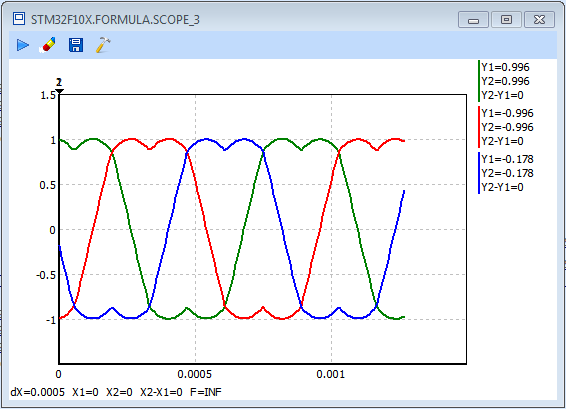
\includegraphics[scale=0.37]{8871_scope}
	\caption{осциллограмма уставок $T_a, T_b, T_c$ от блока в котором не использовались переходы к декартовой системе}
	\label{our_scope}
\end{figure}

%\lstset{caption={Код блока},label={Nechto}}
%\lstinputlisting[linerange={8-91}]{Nechto_a1.c}

%\begin{figure}[!ht]
%\centering
%%\input{AB1}
%        \caption{Изображающий вектор в системах координат в фазах АВ и фазах BC}
%\end{figure}
%В системе координат, образованных фазами B и C: $\vec{u} = u^B \vec{e_B} + u^C \vec{e_C} $

Решены следующие задачи:
%\begin{itemize}
%\item 

-- предоставлена возможность пройти лабораторные удаленно;

-- использовано российское программное обеспечение МехБиос и в ряде демонстраций российский микроконтроллер K1921VT01;

-- упрощено управление электрической машиной в котором отсутствуют лишние переходы в декартову систему и обратно.
%\end{itemize}

\begin{thebibliography}{5}
        \bibitem{Gorev}Горев А.А. Переходные процессы синхронной машины. -- М.,Л., Гос. энергетическое изд., 1950. -- 551 c.
        \bibitem{Sokolovsky}Соколовский Г.Г. Электроприводы переменного тока с частотным регулированием: Учебник для студ. высш.учеб.заведений.
                -- М. «Академия», 2007 - 272 с.
%        \bibitem{Proshivka}Заливка прошивки в STM32 через USB \url{https://habr.com/post/403007/}
%        \bibitem{Zagruzchik}Программа-загрузчик \url{github.com/rogerclarkmelbourne/Arduino\_STM32}
	\bibitem{MexBios}Мехбиос [Электронный ресурс]. -- Режим доступа: URL: \url{http://www.mechatronica-pro.com/ru/catalog/software-0}
	\bibitem{K192101VT}Микроконтроллер K192101VT  [Электронный ресурс]. -- Режим доступа: URL: \url{https://niiet.ru/product/}
	\bibitem{CodeBlock}C-код блока преобразования фазных токов [Электронный ресурс]. -- Режим доступа: URL: \url{https://github.com/trot-t/RemoteLabs}
%        \bibitem{controlSUITE} \url{https://www.ti.com/tool/CONTROLSUITE}
                %описание на русском https://habr.com/post/403007/\\
%на английском %http://www.rogerclark.net/stm32f103-and-maple-maple-mini-with-arduino-1-5-x-ide/
%
%       Сама  программа загрузчик -- \\
%{\small https://github.com/rogerclarkmelbourne/Arduino\_STM32}
\end{thebibliography}
\end{document}

